\documentclass{article}
\usepackage{graphicx} % Required for inserting images
\usepackage[margin=1in]{geometry}
\usepackage{amsmath}
\usepackage{amsthm}
\usepackage{amssymb}
\usepackage{amsfonts}
\usepackage{verbatim}
\usepackage{xcolor}

\title{Homework 4: Report}
\author{Dante Buhl}
\date{Feb. $26^{th}$ 2024}


\DeclareMathOperator{\cond}{cond}
\DeclareMathOperator{\vecspan}{span}

\begin{document}

\newcommand{\bs}[1]{\boldsymbol{#1}}
\newcommand{\bmp}[1]{\begin{minipage}{#1\textwidth}}
\newcommand{\emp}{\end{minipage}}
\newcommand{\R}{\mathbb{R}}
\newcommand{\C}{\mathbb{C}}
\newcommand{\N}{\mathcal{N}}
\newcommand{\I}{\mathrm{I}}
\newcommand{\K}{\bs{\mathrm{K}}}
\newcommand{\m}{\bs{\mu}_*}
\newcommand{\s}{\bs{\Sigma}_*}
\newcommand{\dt}{\Delta t}
\newcommand{\tr}[1]{\text{Tr}(#1)}
\newcommand{\Tr}[1]{\text{Tr}(#1)}

\maketitle


\setcounter{section}{1}

\section{Cholesky Solution of the least-squares problem}
\begin{enumerate}
\item How does the Cholesky Decomposition Work?

The cholesky decomposition is merely a special case of the LU factorization method. It is designed to create a matrix $L$ such that $LL* = A$. That is, we find that $L$ is (with abuse of notation) a "square-root" of $A$ in matrix form. The algorithm is very simple, we start with the $l_{11}$ component of $L$. We have that $l_{11} = \sqrt{a_{11}}$. We proceed just like LU factorization except that the symmetry of $A$ allows us to perform half of the computations necessary (this is due to the symmetry of the problem). You can throw away half of the matrix $A$ (above the diagonal) upon entry and L wouldn't change. 

\item The results of fitting a third degree polynomial are a frobenius norm of error at $||E||_F = 0.19127$. The coefficients build the following polynomial, 
    \[
        f(x) = 0.578 + 4.666x - 10.935 x^2 + 7.514x^3
    \]
    Here is the corresponding plot with that polynomial. 
    
    \bmp{.95}
        \centering
        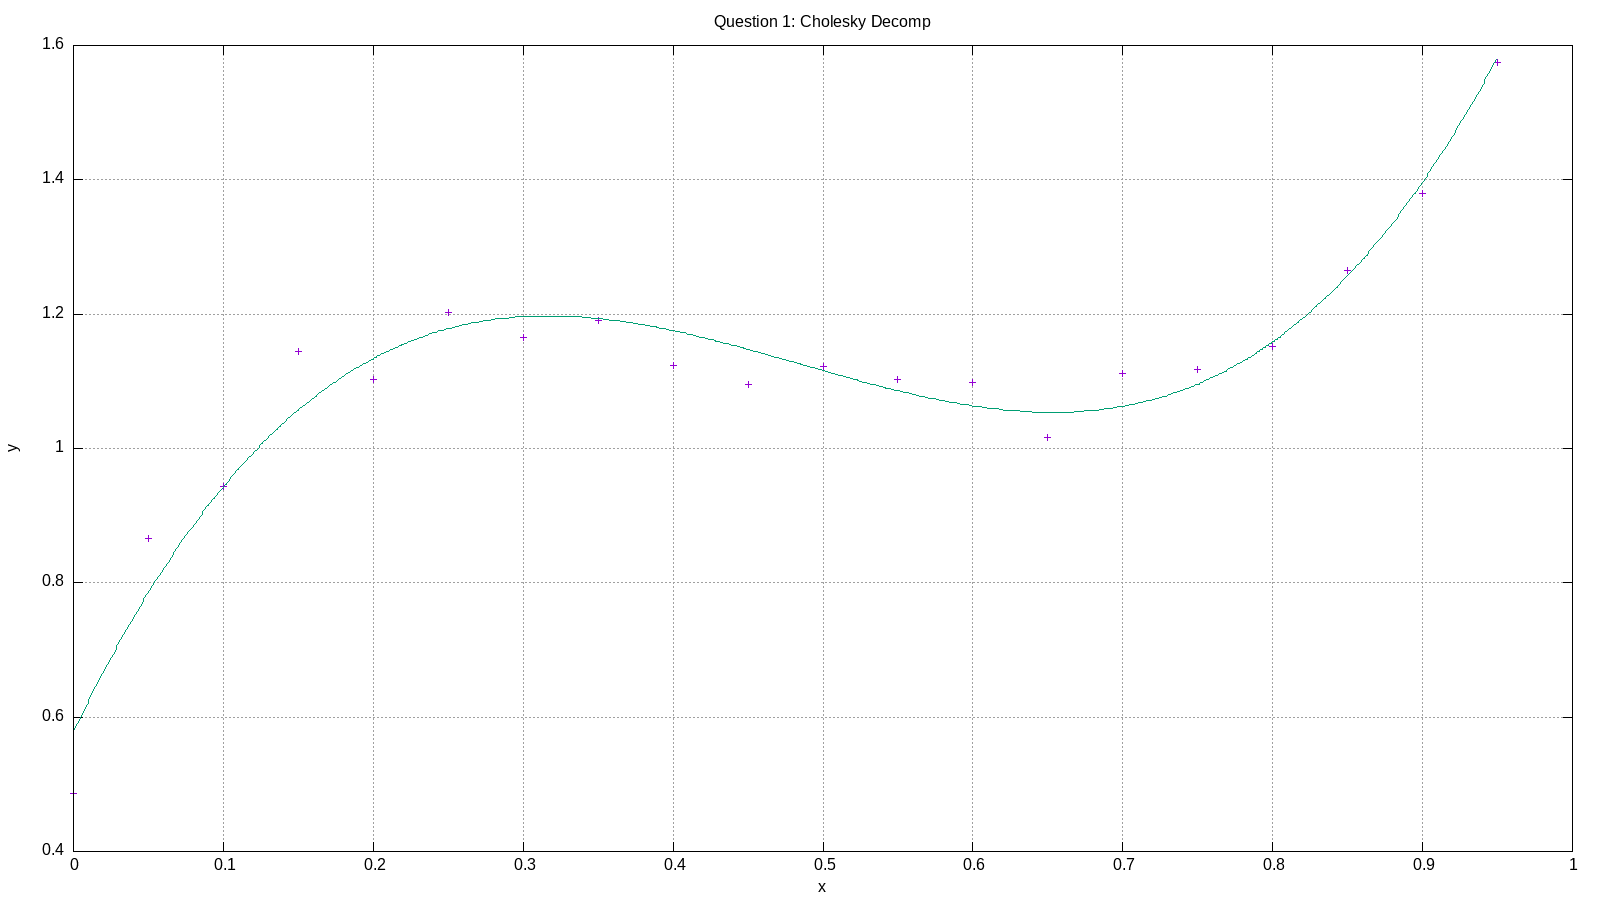
\includegraphics[width=0.7\textwidth]{../fortran/cholesky3plot.png}
    \emp

\item The results of fitting a fifth degree polynomial are a frobenius norm of error at $||E||_F = 0.1418$. The coefficients build the following polynomial, 
    \[
        f(x) = 0.517 + 6.868x - 25.861x^2 + 44.908x^3 - 39.406x^4 + 14.816x^5
    \]
    Here is the corresponding plot with that polynomial. 
    
    \bmp{.95}
        \centering
        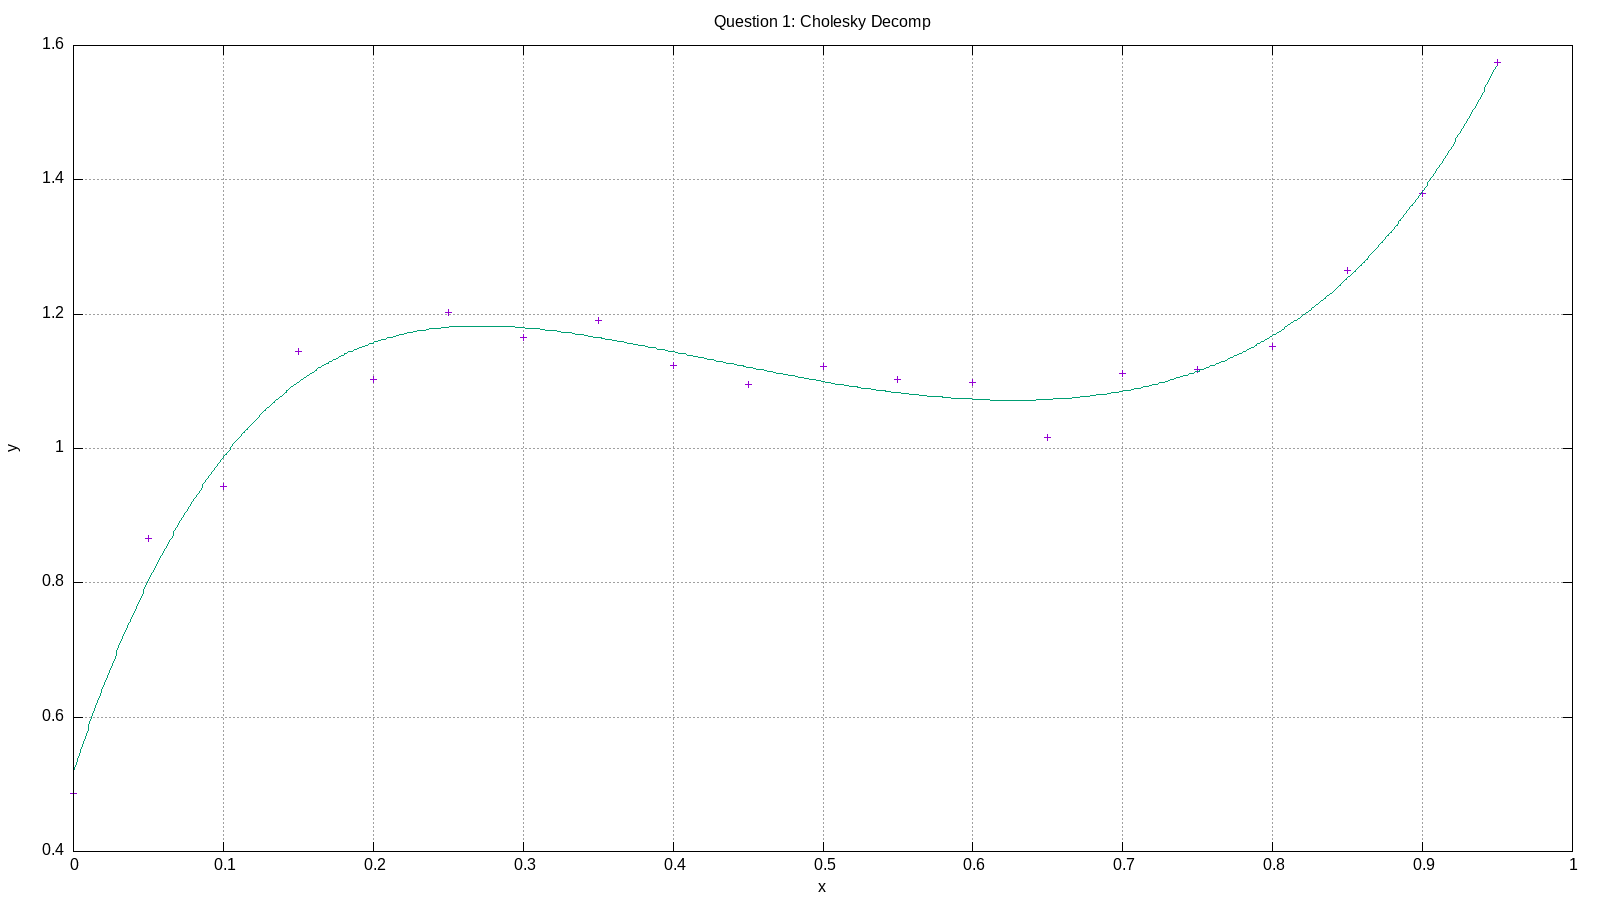
\includegraphics[width=0.7\textwidth]{../fortran/cholesky5plot.png}
    \emp

\item Analytically, the maximum degree of this polynomial should be a ninteenth degree polynomial. Note that if we are solving with a 19th degree polynomial, that we have 20 equations with 20 unknowns. There should be one exact solution. As soon as there are more than 20 unknowns (i.e. 20+ degree polynomial), we now have an underdetermined system. Thus we cannot solve for all of the coefficients. Numerically, it is even less due to the nature of this domain of data and machine precision accuracy.

\item 
    The algorithm fails in single precision when one of the columns is filled with machine precision zero. The reason why is that at higher degree polynomials, we are taking an x value between 0 and 1, and raising it to a very high power. Take for example $x = 0.65$. We have, 
    \[
        x= 0.65, \quad x^{n} = 6.5^{n} \cdot 10^{-n}
    \]
    It becomes evident fairly quickly, that since $10 > 6.5$ that as n becomes large that $x^n$ will decay to zero, more specifically machine precision zero. For a data set $S$ with $x \in [0, 1)$ we will have that there is a value of $n$ large enough such that $x^n \le \epsilon_{\text{mach}}, \forall x \in S$. Once an entire column of the vandermonde matrix is machine precision zero, we will have that the matrix becomes singular and we can no longer perform a regression.  

\end{enumerate}

\section{QR Solution of the least-squares problem}
\begin{enumerate}
\item  Explain how the Householder QR method works. 
    
    The householder QR method works by considering an orthogonalization of $A$. The method works by constructing $Q_i$ a block matrix containing an identity matrix and a householder reflector. We have that at each iteration, the columns of $A$ become orthogonalized in the following way.  $A_{i-1}$ is a matrix with zeros under the diagonal for columns $1, i-1$. When multplying by $Q_i$ we obtain a matrix now with zeros underneath the diagonal for columns $1, i$ and the column vectors of the block matrix $A_{i:m, i+1:n}$ are all orthogonal to $A_{i:m, i}$. By repeating this for all columns of $A$ we obtain the unitary matrix $Q = Q_1\cdots Q_n$ and the resulting matrix $Q^*A$ is an upper triangular matrix (with exception for the fact that it is rectangular). That is, $Q^*A = R = \left[\begin{array}{c} \hat{R} \\ 0\end{array}\right]$. 
    \[
        Q_i = \left[\begin{array}{c c} \I & 0 \\ 0 & H_i \end{array}\right], \quad 
        Q_iA_{1:m, i} = \left[\begin{array}{c}a_{1} \\ \vdots\\ a_{i}' \\ 0 \\ \vdots\\ 0 \end{array}\right]
    \]

\item 3rd degree

The results of fitting a fifth degree polynomial are a frobenius norm of error at $||E||_F = 0.1912$. The coefficients build the following polynomial, 
    \[
        f(x) = 0.578 + 4.666x - 10.936x^2 + 7.514x^3
    \]
    Here is the corresponding plot with that polynomial. 
    
    \bmp{.95}
        \centering
        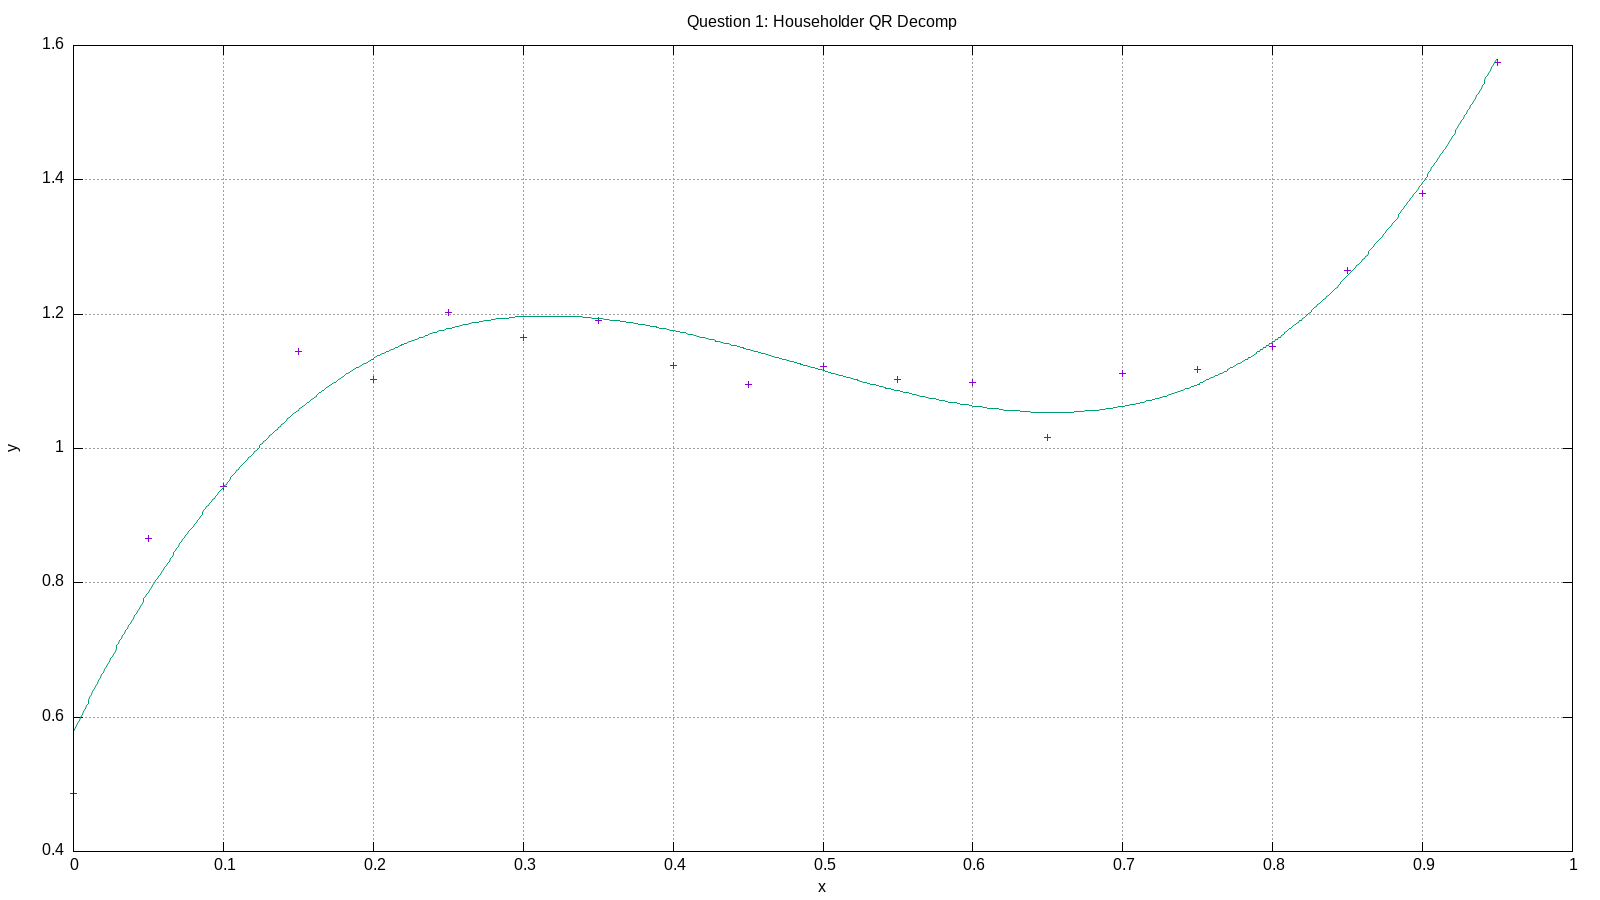
\includegraphics[width=0.7\textwidth]{../fortran/qr3plot.png}
    \emp

\item 5th degree

The results of fitting a fifth degree polynomial are a frobenius norm of error at $||E||_F = 0.1403$. The coefficients build the following polynomial, 
    \[
        f(x) = 0.509 + 7.248x - 28.818x^2 + 53.261x^3 - 49.206x^4 + 18.878x^5
    \]
    Here is the corresponding plot with that polynomial. 
    
    \bmp{.95}
        \centering
        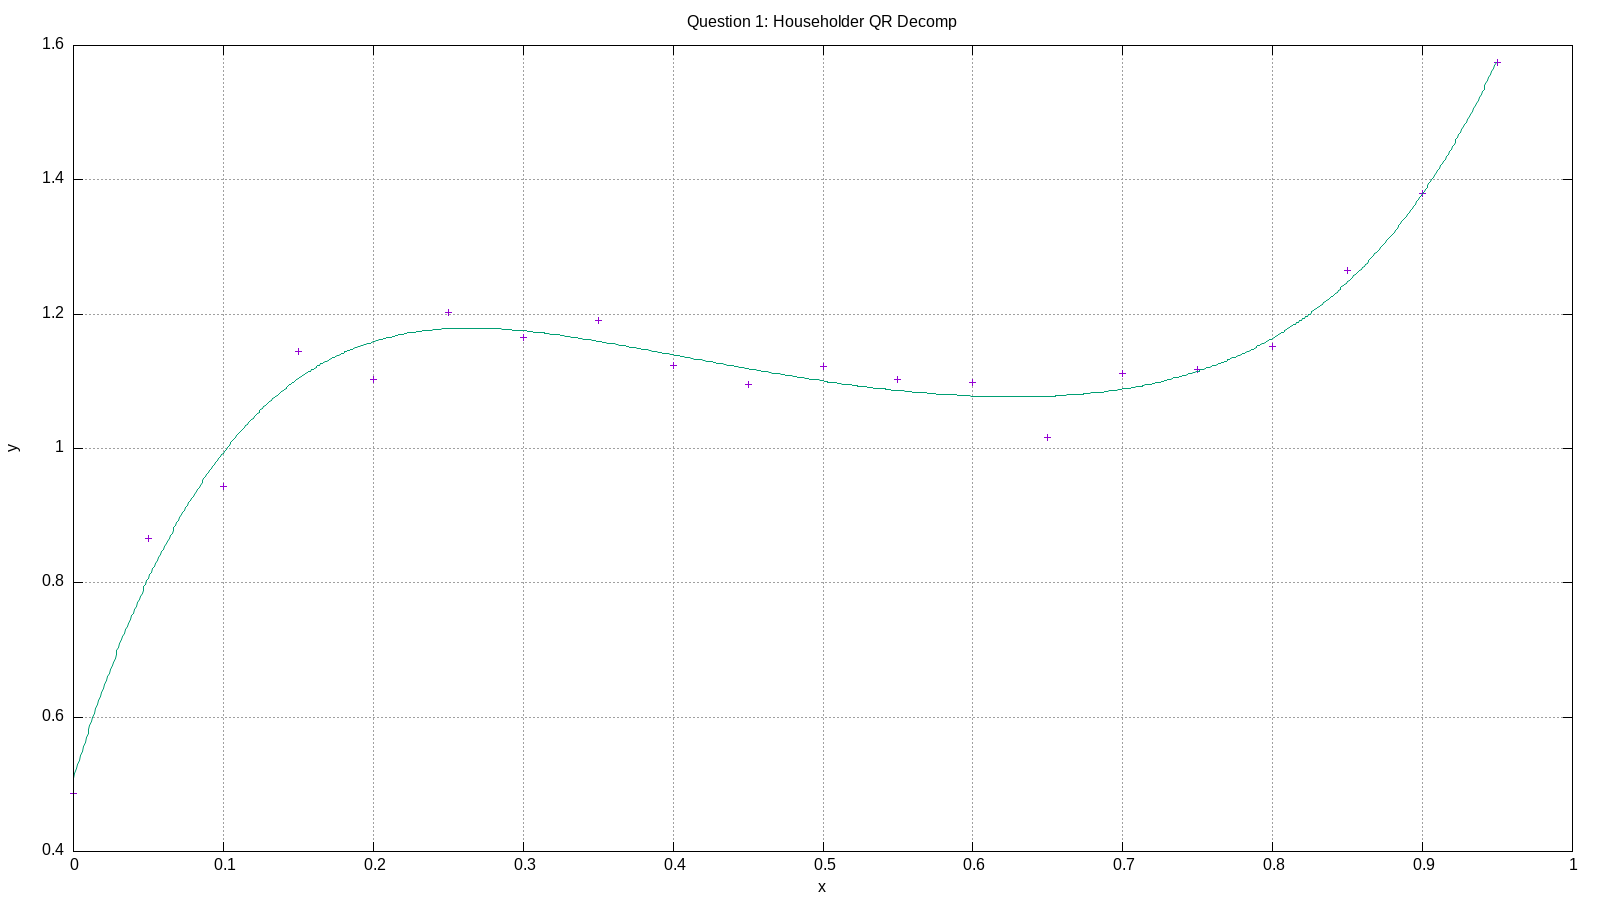
\includegraphics[width=0.7\textwidth]{../fortran/qr5plot.png}
    \emp

\item When does it fail?
    
The QR method seems to hold up very long in single precision. It makes a reasonable regression all the way up to a 13th degree polynomial. Note that the plot looks very bad at this degree of polynomial as the numerical precision of calculating any term of degree 10 or more is very choppy. This is similar to the plotting issue seen in the first or second homework (plotting $(x-9)^8$ was much better than the expanded form). Also note that Cholesky Method begins to fail in single precision starting at 7th degree polynomials. It lasts much longer in double precision. In fact, one could even claim that the $QR$ method will continue to work all the way out to a ninteeth degree polynomial. Notice that at this degree, the regression is not smooth due to the same plotting errors and is also generally inaccurate, but it returns all real, finite coefficients. It can be argued whether QR fails, but compared to the cholesky method at this degree of polynomial (which returns all NAN for the coefficients) it is much better.

\item For 5th order discuss, $A - QR$, $Q^TQ - I$. 
    
The error is as expected for single precision code. We get errors at orders of $10^{-6}$-$10^{-7}$. This is expected since sinple precision machine zero is $10^{-7}$. For double precision the error is at order $10^{-15}$. 
    \[
        ||A-QR||_F \approx 1.042\cdot10^{-6}, \quad ||Q^TQ - \I||_F \approx 6.398\cdot10^{-7}
    \]

\end{enumerate}

\section{Theory Problems}
\begin{enumerate}

\item %start of problem 1
Show that is $P$ is an orthogonal projector, then $\I - 2P$ is unitary. 

\begin{proof}
    We begin with the definition of a unitary matrix. We have a unitary matrix $Q$ is a matrix such that $Q^*Q = \I$. We now look for this quality in $(\I - 2P)$. 
    \[
        (\I - 2P)^*(\I - 2P) = (\I - 2P^T)(\I - 2P) = (\I - 2P)(\I - 2P)
    \]
    The above quality $P^T = P$ is from the fact that $P$ is an orthogonal projector. We also have the quality that $P^2 = P$.
    \[
        (\I - 2P)(\I - 2P) = \I(\I - 2P) - 2P(\I - 2P) = \I - 2P - 2P + 4P^2
    \]
    \[
        = \I - 4P +4P = \I
    \]  
    We have recovered the condition for unitary matrices. We can therefore declare $(\I - 2P)$ a unitary matrix. 
\end{proof}


\item % start of problem 2
Let $P \in \R^{m \times m}$ be a nonzero projector. 
\begin{enumerate}
    \item Show that $||P||_2 \ge 1$, with equality if and only if $P$ is an orthogonal projector. 
    \begin{proof}
        (i) without equality
        
        We begin by looking at a projector $P$ which transforms a vector onto the span of another unit vector $v$. That is $P: \R^m \to \vecspan(v)$. We look at the case of the definition of the two-norm for matrices. 
        \[
            ||P||_2 = \sup_{x} \frac{||Px||_2}{||x||_2}
        \]
        We now take the case $x = v$. 
        \[
            ||P||_2 = \sup_{x} \frac{||Px||_2}{||x||_2} \ge \frac{||Pv||_2}{||v||_2}
        \]
        We notice that $v \in \vecspan(v)$, so the transformation $P$ is the identity for $v$. So, 
        \[
            ||P||_2 \ge \frac{||Pv||_2}{||v||_2} = \frac{||v||_2}{||v||_2} = 1
        \]
        \[
            ||P||_2 \ge 1
        \]

        (ii) with equality ($\implies$)
    
        We now look more closely at the definition of $P$ and the singular value decomposition of $P$. If $P$ is orthogonal we have that $P = vv^T$ for some unit vector $v \in \R^m$. We also have by the singular value theorem, that a singular value will satisfy the following property, 
        \[
            Pv_i = \sigma_iu_i, \quad P = U\Sigma V^T
        \]
        Where we have that $v_i, u_i$ are the i-th column vectors of $V, U$ respectively, and $\sigma_i$ is the i-th diagonal element of $\Sigma$. Note that $U, V$ are unitary and as a consequence its column vectors are orthogonal and have two-norm of 1. We look at some $P = xx^T$ for a unit vector $x$. 
        \[
            Pv_i = \sigma_iu_i \to xx^Tv = \sigma_iu_i
        \]
        \[
            (x, v_i) x = \sigma_i u_i
        \]
        We notice that vectors $x, u_i$ are related by scalars as a consequence of this definition of $P$. Therefore $x$ and $u_i$ must be colinear, however this is not guaranteeed by our assumptions. We have a few consequences and cases. Either $x$ and $u_i$ are colinear, or they are not. We look at the case they are colinear, 
        \[
            x = \alpha u_i
        \]
        We then must have that $\alpha = \frac{\sigma_i}{(x, v_i)}$. We then look at one of our prior assumptions. We have most importantly that $||x||_2 = ||v_i||_2 = ||u_i||_2 = 1$. 
        \[
            ||x||_2 = |\alpha|||u_i||_2 = 1, \implies |\alpha| = 1
        \]
        \[
            \sigma_i = \pm (x, v_i)
        \]
        We need two more things. First, that singular values cannot be negative by definition. Second, we have that if both $x$, $v_i$ are unit vectors, we cannot have that their inner product is greater than 1. Another way of expressing this is the geometrical interpretation that the dot product is $x \cdot v_i = (x, v) = ||x||_2||v_i||_2\cos(\theta)$. If $||x||_2 = ||v_i||_2 = 1$, $(x, v_i) = \cos(\theta) \le 1$. Finally, (and I mean it this time), we look at the case where $Px = x$ we have that since $x$ is a unit vector we recover an eigenvalue (in this case also a singular value) of $P$. Thereby we officially have, 
        \[
            0 < \sigma_i \le 1, \sigma_1 = 1
        \] 
        We use a proof from a different homework problem (or maybe from the lecture note, I can't remember where) relating $||A||_2 = \sigma_1$, to show, 
        \[
            ||P||_2 = \sigma_1 = 1
        \]

        ($\impliedby$) If $||P||_2 = 1$, then $P$ is an orthogonal projector (i.e. $P^T = P$)

        We begin by looking at the definition of the two norm for matrices. We have, 
        \[
            ||P||_2 = \sup_{x} \frac{||Px||_2}{||x||_2} = 1
        \]
        Therefore the case exists such that we find, 
        \[
            ||Px||_2 = ||x||_2
        \]
        We then introduce the fact that a two norm of a vector is the square root of the inner product of that vector with itself. That is $||v||_2 = \sqrt{(v, v)}$. Thus we have, 
        \[
            \sqrt{x^TP^TPx} = \sqrt{x^Tx}
        \]
        \[
            x^TP^TPx = x^Tx
        \]
        \[
            P^TPx = x = PPx, \quad \text{by definition of a projector}
        \]
        \[
            P^TPx = PPx, \implies P^Ty = Py
        \]
        This implies that for any vector in the span of $v$ (We take $P: \R^m \to \vecspan(v)$), that $P^T = P$. Moreover we have that for any vector $x$, $P^TP = P^2$. If we take $P$ to be invertible, we have that $P^T = P$. Therefore, we have that $P$ is idempotent and symmetric, making it an orthogonal projector. 
        
    \end{proof}

    \item Show that if $P$ is an orthogonal projector, then P is semi-positive deinite with its eigenvalues either zero or 1. 
        \begin{proof}
            We look at the vector product definition of $P$. $P = xx^T$ for a unit vector $x$. 
            \[
                (v, Pv) = v^Txx^Tv = (v, x)(x, v) = (x, v)^2 \ge 0
            \]
            Since our choice of $v$ was arbitary we have that $P$ is semi-positive definite. 
            
            Next we look at the eigenvalues of $P$. Say that we have an arbitary eigenvalue-eigenvector pair ($\lambda, v$) for $P$ such that $v \neq \vec{0}$ (obviously). We have,
            \[
                Pv = \lambda v
            \]
            \[
                Pv = xx^Tv = (x, v)x = \lambda v
            \]
            Notice that $(x, v)$ and $\lambda$ are scalars. This implies that $x$ and $v$ are colinear but this was not an assumption made. Therefore we are left with two cases: $v$ and $x$ are colinear, or $v$ and $x$ are orthogonal. Let's look at the first case, $v = \alpha x$.
            \[
                (x, v)x = \alpha x = \alpha\lambda x
            \] 
            \[
                x = \lambda x \implies \lambda = 1
            \]
            We find that for all vectors colinear to $x$ are eigenvectors with eigenvalue 1. We look at the other case. If $x$ and $v$ are orthogonal we have $(x, v) = 0$. 
            \[
                \vec{0} = \lambda v \implies \lambda = 0
            \]
            Therefore all vectors orthogonal to $x$ will be eigenvectors with $\lambda = 0$. 
        \end{proof}
\end{enumerate}

\item   % start of problem 3
Let $A \in \R^{m \times n}$ with $m \ge n$, and let $A = \hat{Q}\hat{R}$ be a reduced $QR$ factorization. 

\begin{enumerate}
\item Show that $A$ has rank $n$ if and only if all the diagonal entries of $\hat{R}$ are nonzero.
    
\begin{proof}
    
    ($\implies$) $A$ is rank $n$ if all of the diagonal entries of $\hat{R}$ are nonzero. 
    
    Let us look at the reduced QR factorization of $A$ such a that all diagonal entries of $\hat{R}$ are nonzero. 
    \[
        A = \hat{Q}\hat{R} = \left[q_1 \Big| \cdots \Big| q_n\right]\hat{R}
    \]
    We have by construction of a QR factorization that the matrix $\hat{Q}$ is composed of orthogonal unit column vectors $q_i$. Let us now look at the column vectors of $A$. 
    \[
        a_i = r_{1i}q_1 + \cdots + r_{ii}q_i
    \]
    Notice that since all diagonal elements of $\hat{R}$ are nonzero that we have that each $a_i$ is immediately distinguished from $a_{i-1}$ by the inclusion of the vector $q_i$. Let us start a small induction proof. Take the base case to demonstrate that $a_1$ is linearly indepentent from $a_2$. By contradiction suppose that $a_1, a_2$ are linearly dependent. 
    \[
        0 = c_1a_1 + c_2a_2 = c_{1}r_{11}q_1 + c_2r_{12}q_1 + c_2r_{22}q_2 = (c_1r_11 + c_2r_{12})q_1 + c_2r_{22}q_2
    \]
    \[
        0 = d_1q_1 + d_2q_2
    \]
    However, since the vectors $q_i$ are linearly independent, we require that $d_1 = d_2 = 0$ since the vectors $q_1, q_2$ are linearly independent. Immediately we notice that $c_2$ must equal zero since $r_{22} \neq 0$. Therefore for the two to be linearly dependent we must have that $c_1 \neq 0$. A contradiction is reached, since $d_1 = 0 = c_1r_{11} + 0 \implies r_{11} = 0$. Thus we have that $a_1, a_2$ are linearly independent. 
    
    Next we look at the inductive step. Take $a_1, \cdots, a_k$ to be linearly independent. Let us look at the set $a_1, \cdots, a_{k+1}$. We have evidently, that, 
    \[
        c_1a_1 + \cdots + c_ka_k = d_1q_1 + \cdots d_kq_k
    \]
    Such that $d_1q_1 + \cdots + d_kq_k = 0$ if and only if $d_1 = \cdots = d_k = 0 = c_1 = \cdots = c_k$. Let us now add $c_{k+1}a_{k+1}$ and look at the linear dependence. 
    \[
        c_1a_1 + \cdots + c_ka_k + c_{k+1}a_{k+1} \] \[(d_1 + c_{k+1}r_{1k})q_1 + \cdots (d_k+c_{k+1}r_{kk+1})q_k + c_{k+1}r_{k+1, k+1}q_{k+1} = 0
    \]
        Again these vectors, $q_i$, are linearly independent so we must have that $c_{k+1} = 0$ since $r_{k+1, k+1} \neq 0$. Therefore we are left with 
    \[
        d_1q_1 + \cdots d_kq_k = 0
    \]
    We already have that to satisfy this, $d_1 = \cdots = d_k = 0$, thereby we have immediately that the vectors $a_1, \cdots, a_{k+1}$ are linearly independent. Therefore, by inductive argument we have that all $n$ vectors $a_i$ constructed this way from the reduced QR factorization will be linearly independent. As a corallary to this finding, we find that $A$ is rank $n$ by the definition of rank and it being that $A$ is composed of $n$ linearly independent column vectors. 
    \vspace{10pt}

    ($\impliedby$) All diagonal entries of $\hat{R}$ are non-zero if $A$ is rank $n$. 

    Assume by the way of contradiction that both $A$ is rank $n$ and that $\hat{R}$ has at least one diagonal entry, $r_{kk} = 0$. 
    We look at the construction and linear dependence of the column vectors of $A$. Look specifically at $a_k$. We have, 
    \[
        a_k = r_{1k} q_1 + \cdots + r_{k-1, k} q_{k-1} + r_{kk} q_k
    \]
    \[
        c_1a_1 + \cdots + c_ka_k = 0
    \]
    Notice that since $r_{kk} = 0$ $a_k$ is only constructed of $q_1, \cdots, q_{k-1}$. 
    \[
        c_1a_1 + \cdots + c_ka_k = (c_1r_{11} + \cdots + c_kr_{1k})q_1 + \cdots + (c_{k-1}r_{k-1, k-1} + c_kr_{k-1, k})q_{k-1} = 0 
    \]
    We must have again that, $d_1 = \cdots = d_{k-1} = 0$. We then chose $c_k = 1$ for simplicity and obtain a system of equations.
    \[
        c_1r_{11} + \cdots + r_{1k} = \cdots =  c_{k-1}r_{k-1, k-1} + r_{k-1, k} = 0
    \]
    Notice that we have $k-1$ equations with $k-1$ unknowns, so we are guaranteed a solution exists such that at least one $c_i \neq 0$. i.e. 
    \[
        c_{k-1} = -\frac{r_{k-1, k}}{r_{k-1, k-1}} 
    \]
    Therefore we have that the set of column vectors $a_1,\cdots, a_k$ are linearly dependent. Therefore, we have at most that $A$ is rank $n-1$ (Take $\{a_1, \cdots, a_{k-1}, a_{k+1}, \cdots a_n\}$ and check their dependency. They may be linearly independent!). Therefore we have reached a contradiction. If $A$ is full rank (rank = $n$) we cannot have that any diagonal elements of $\hat{R}$ are zero as it would reduce the rank of $A$ by at least one. If $A$ is full rank, $\hat{R}$ must have nonzero diagonal entries. 

\end{proof}

\item Suppose $\hat{R}$ has $k$ nonzero diagonal entries for some $k$ with $0 \le k < n$. What does this imply about the rank of $A$? Exacktly $k$? At least $k$? At most $k$? Give a precise answer and prove it.

    \begin{proof}

    (Case: rank $k$) 

    The goal is to show with two cases that such a matrix can be constructed with rank $n-1$ and one with rank $k$. Therefore stating that the rank of $A$ is at least $k$.  
    Let us look at the case where $\hat{R}$ is a matrix composed of zeros entirely except for $k$ entries along the diagonal.
    \[
        A = \hat{Q}\hat{R}
    \]
    \[
        A = \left[ a_1 \Big | \cdots \Big | a_n \right]
    \]
    Notice that only $k$ column vectors of $A$ are nonzero by this construction of $A$, and $\hat{R}$. Therefore the column vectors which are zero vectors are not linearly independent with each other nor the nonzero column vectors of $A$. So we must have that there are $k$ linearly independent column vectors in $A$. Therefore $A$ is rank $k$. To demonstrate this formally we have
    \[
        c_1a_1 + \cdots c_na_n = \sum_{i, r_{ii} \neq 0} c_ir_{ii}q_i = 0
    \]
    We must have by the linear independence of $q_i$ that $c_ir_{ii} = 0$ for this to be true, but then $c_i = 0$. Since there are $k$ terms in this sum, there are therefore $k$ linearly independence vectors in $A$. 

    (Case: rank $n-1$)

    We next take a case for $\hat{R}$ that will produce $A$ rank $n-1$. We chose an $\hat{R}$, complete with k nonzero entries on the diagonal and zero's above the diagonal for those $k$ columns. For the columns with zero's on the diagonal we demonstrate a particular form for them. For the first column with a zero on the diagonal, the form is not very important. Suppose this is column $i$. Look at the next column with a zero on the diagonal, suppose it is column $j$.  Let column $j$, $r_j$ be of the following form.
    \[
        r_j = \left[\begin{array}{c}
                    0 \\
                    \vdots  \\
                    0 \\
                    r_{i, j} \\
                    0 \\
                    \vdots \\
                    0 
                    \end{array}\right]
    \] 
    These columns are such that if column $c_j$ was in the $i-th$ column rather than the $j-th$ it would resemble an diagonal matrix with nonzero diagonals except for the very last column with one zero on the diagonal (lets denote this column $r_z$). That is, if we permuted the columns of $\hat{R}$ we could obtain a matrix $\hat{R}'$ such that only one column of $\hat{R}'$ has a diagonal entry of zero.  This would produce a matrix $A'$ with the corresponding columns permuted in the same way. Notice however, that $A'$ has the same rank as $A$. That is, it contains the same column vectors, just in a different order. Notice that besides the one column with a zero along the diagonal (lets call this column $a_z$), we have that $\hat{R}'$ is a diagonal matrix. Therefore we have the columns of $A'$ are such that, 
    \[
        a_i' = r_{ii}'q_i, \quad  a_z = r_{1z}'q_1 + \cdots + r_{z-1z}'q_{z-1}
    \]
    We have that $r_{ii}' \neq 0$, so 
    \[
        \sum_{1 \le i \le n, i \neq z} c_ia_i' = \sum_{1 \le i \le n, i \neq z} d_1q_i = 0, \quad (d_i \propto c_i), \quad \text{iff}  \quad c_i = 0, \quad  \forall i
    \]
    Notice that this linear combination (sum) has $n-1$ terms in it, therefore we have that $A'$ is rank $n-1$ and therefore so is $A$. This ultimately implies that the rank of $A$ is bounded on the lower end by $k$ and on the upper end by $n-1$. 
    \end{proof}
\end{enumerate}


\item % start of problem 4
Determine the (i) eigenvalues, (ii) determinant, and (iii) singular values of a Householder reflector. For the eigenvalues, give a geometric argument as well as an algebraic proof. 

\begin{proof}
    (i) Eigenvalues 

    We start with the definition of a householder reflector for a unit vector $x$. Take $H = \I - 2xx^T$ with an eigenvalue-eigenvector pair ($\lambda, v$) such that $Hv = \lambda v$. 
    \[
        Hv = (\I - 2xx^T)v = v - 2xx^Tv = v - 2(x, v)x = \lambda v  
    \]
    \[
        -2(x, v) x = (\lambda - 1) v
    \]
    We again have a case where $x$ and $v$ are vectors connected by scalar arguments. We must have that $x$ and $v$ are colinear. We take the two cases, $x$ and $v$ are colinear, $x$ and $v$ are orthogonal. 
    \[
        v = \alpha x, \quad -2(x, v) = -2\alpha
    \]
    \[
        -2\alpha = (\lambda - 1) \alpha 
    \]
    \[
        \lambda = -1
    \]
    Therefore if $x$ and $v$ are colinear we have that $v$ is an eigenvector of $H$ and that its eigenvalue is $\lambda = -1$. We look at the next case, $x$ and $v$ are orthogonal, therefore $(x, v) = 0$. 
    \[
        -2(0)x = (\lambda - 1)v \implies \lambda - 1 = 0
    \]
    \[
        \lambda = 1 
    \]
    Therefore we have that if $x$ and $v$ are orthogonal that the eigenvalue corresponding to $v$ is equal to 1. 
    \vspace{5pt}

    (ii) Determinant 

    Next we look at the determinant of $H$. We have that from exercise one that $H$ is unitary (orthogonal) and symmetric. Therefore (going in one direction) that $H^{-1} = H^*$. This is because $H^*H = \I = H^{-1}H$. Next we also have that for any matrix A, $\det(A^*) = \overline{\det(A)}$. We also have that, $\det(A)\det(A^{-1}) = 1$.
    \[
        \det(H^{-1}H) = \det(H^{-1})\det(H) = 1
    \]
    \[
        \overline{\det(H)}\det(H) = 1 
    \]
    \[
        \det(H)^2 = 1 \implies \det(H) = \pm 1
    \]
    
    (iii) Singular Values

    We have from the proof in exercise one, we have that $H \in \R^{m\times m}$ is a unitary (orthogonal) matrix. We have therefore that $H$ preserves the length of vectors under transformation. We also look at the singular value decomposition of $H$. 
    \[
        H = U\Sigma V^T, \quad ||Hv|| = ||v||, \forall v \in \R^{m}
    \]
    Let us look at a specific vector $v_i$ now such that $v_i$ is i-th column vector of $V$. 
    \[
        ||Hv|| = ||U\Sigma V^Tv_i|| = ||u_i\sigma_{ii}|| 
    \]
    We recover the scalar-vector product, $u_i\sigma_{ii}$ where $u_i$ is the i-th column vector of $U$ and $\sigma_{ii}$ is the i-th diagonal element of $\Sigma$. We return to the fact that by the Singular Value Decomposition Theorem, that $U, V$ are unitary, that is they are composed of orthogonal column vectors with norm of 1. Therefore we have, 
    \[
        ||Hv|| = ||v_i|| = ||\sigma_{ii}u_i|| = |\sigma_{ii}|||u_i||
    \]
    \[
        1 = |\sigma_{ii}|1, \implies \sigma_{ii} = \pm 1
    \]
    Therefore since our choice of $v$ was arbitrary among the column vectors of $V$ we have that this example exhausts all singular values for $H$. Thus the singular values of $H$ are $\pm 1$. It can even be argued that the plus minus in this context does not matter. Since singular values are scalars which in a transformation from one vector basis to another scale the vector in the resulting basis. The vectors in the output basis are orthogonal so scaling one vector say by $-1$ would not make that basis linearly dependent. Therefore we claim that any $u_i$ will absorb the sign of $\sigma_{ii}$ (Also because of the fact that singular values are always positive). So it is as simpler to claim that, 
    \[
        \sigma_{ii} = 1.
    \]
    Therefore the singular values of $H$ are such that, $\sigma_{ii} = \sigma_i = 1$. 
\end{proof}

\item  % start of problem 5
Let $A \in \R^{m\times n}$. Show that $\cond(A^TA) = \left(\cond(A)\right)^2$. 

    \begin{proof}
        We start with the singular value decomposition of $A$. 
        \[
            A = U\Sigma V^T, \quad U, V \text{ unitary}
        \]
        \[
            A^TA = V\Sigma U^T U \Sigma V^T = V\Sigma^2V^T
        \]
        Notice that this is a singular value decomposition for $A^TA$ since $V, V^T$ are unitary matrices and $\Sigma^2$ is a diagonal matrix with positive or zero entries along the diagonal. We look at the fact that the condition number of a matrix $A$ is  proportional to the two norms of $A$ and $A^{-1}$. 
        \[
            \cond(A^TA) = ||A^TA||_2 \cdot ||(A^TA)^{-1}||_2
        \]
        We will also use the fact that the two-norm of a matrix is equal to its largest singular value. We now look for $(A^TA)^{-1}$. 
        \[
            (A^TA)^{-1} (A^TA) = \I
        \]
        \[
            U_1U_2U_3 V \Sigma^2V^T = \I
        \]
        Very evidently from this assumption we can pick three matrices to invert $A^TA$. We take $U_3 = V^T$, $U_2 = \Sigma^{-2}$ (this inverse exists because $\Sigma$ is diagonal), $U_1 = V$ (assuming that $V$ is invertible). Thus we have, 
        \[
            (A^TA)^{-1} = V\Sigma^{-2}V^T
        \]
        Notice that this is also a singular value decomposition for $(A^TA)^{-1}$ since both $V, V^T$ are unitary and $\Sigma^{-2}$ is still diagonal. Notice however the largest singular values for $A^TA, (A^TA)^{-1}$ are $\sigma_1^2, \frac{1}{\sigma_k^2}$ respectively. Therefore we go back to the condition number. 
        \[
            \cond(A^TA) = ||A^TA||_2 \cdot ||(A^TA)^{-1}||_2 = \sigma_1^2 \frac{1}{\sigma_k^2} = \left(\frac{\sigma_1}{\sigma_k}\right)^2 = \left(\cond(A)\right)^2
        \]  
        This last bit ($\cond(A) = \frac{\sigma_1}{\sigma_k}$) is taken from a proof in lecture (I don't know where but its fairly evident using a singular value decomposition in almost exactly the same way as we are presenting this argument). 
   \end{proof}

\end{enumerate}

\end{document}
